\section{A local activity-feedback model for coupling gains}
\label{sec:localgainsupp}

\subsection{Pairwise exchange replaces a global comparison}

Let \(b_i\) be a route's target excess variance, with \(b_i\geq0\)
and \(\sum_i b_i=B\). The routes exchange this target budget along
a connected graph with symmetric weights \(w_{ij}\geq0\). When
the realized cost \(x_i=\kappa_i m_i^2\) tracks \(b_i\) exactly,
the rule is
\begin{equation}
  \dot b_i=\eta\sum_j w_{ij}[\pi_j(b_j)-\pi_i(b_i)].
  \label{eq:edgefeedback}
\end{equation}
Here \(\pi_i\) is the expected correctness probability defined in
Sec.~\ref{sec:feedbacksupp} for a fixed readout window. Exchange
on an edge cancels from the total budget. At a zero budget the
correctness probability is at chance, so the field does not point
out of the simplex. With \(V(\boldsymbol b)=\sum_i\int_0^{b_i}
\pi_i(u)\,\dd u\),
\begin{equation}
 \dot V=-\frac{\eta}{2}\sum_{ij} w_{ij}(\pi_i-\pi_j)^2.
\end{equation}
On the fixed-budget plane, uniqueness of trajectories also follows
from contraction in the quadratic distance defined by the Laplacian
pseudoinverse: the derivative of half that distance squared for two
solutions is \(-\eta\sum_i(b_i-\widetilde b_i)
[\pi_i(b_i)-\pi_i(\widetilde b_i)]\leq0\). By connectedness,
zero dissipation requires all outputs to have equal correctness.
On the compact simplex this gives global convergence to the unique
max--min allocation, by the common-target argument in
Sec.~\ref{sec:feedbacksupp}. No node needs the global mean correctness.
The network is given a total target budget through initialization;
it does not learn the value of \(B\).

\subsection{Estimating the cost and adjusting the actual gain}

The source-driven component of the output under a fixed unit
gain satisfies \(\dot r_i=D_i r_i+B_i u_i\).
If the output-local noise is independent of the source noise,
then in stationarity \(v_i=v_i^{\rm local}+m_i r_i\), and
\begin{equation}
 \kappa_i=\Tr\operatorname{Cov}(r_i),\qquad
 \tau_\kappa\dot{\hat\kappa}_i=\|r_i\|^2-\hat\kappa_i,
 \qquad
 \dot m_i=\gamma(b_i-\hat\kappa_i m_i^2).
 \label{eq:gainhomeostasis}
\end{equation}
The variance estimate uses zero-mean cue-free activity. The filter
must represent the source-driven response, not total output activity;
for a recurrent module it requires access to the incoming drive and
a copy of the output filter, potentially with several state variables.
Neither the analytic coefficient \(\kappa_i\) nor the optimal gain
enters the updates. At a positive fixed \(b_i\) and exact cost
estimate, the gain drifts monotonically toward
\(\sqrt{b_i/\kappa_i}\) from either side. At \(m_i=0\) it has finite
derivative \(\gamma b_i\). The actuator changes the forward block
only, so it leaves the frozen neural decay spectrum unchanged.
This does not imply that the covariance during adaptation is
stationary. In particular, \(\sum_i b_i\) is conserved, but the sum
of the frozen-gain costs \(\sum_i\kappa_i m_i^2\) need not be
exactly \(B\) while the gains are adjusting.

For the deterministic mean model, let the edges compare the
stationary readout probabilities \(\pi_i(x_i)\) at the actual gains.
At the interior optimum with
\(\hat\kappa_i=\kappa_i\), the budget and realized costs agree.
Write \(y=\delta\boldsymbol x\), \(z=\delta\boldsymbol b\),
\(H=\operatorname{diag}(\pi_i'(x_i^*))>0\),
\(G=\operatorname{diag}(2\gamma\kappa_i m_i^*)>0\), and let
\(L\) be the symmetric graph Laplacian. The linearized equations
at fixed cost estimates are \(\dot z=-\eta LH y\) and
\(\dot y=G(z-y)\). Eliminating \(z\) yields
\begin{equation}
 HG^{-1}\ddot y+H\dot y+\eta HLHy=0,
 \qquad \mathbf{1}^{\mathsf T}(y+G^{-1}\dot y)=0 .
\end{equation}
The energy \((\dot y^{\mathsf T}HG^{-1}\dot y+
\eta y^{\mathsf T}HLHy)/2\) decreases at rate
\(-\dot y^{\mathsf T}H\dot y\). On the constrained subspace it is
positive definite: its only possible zero has \(\dot y=0\),
\(Hy\) constant, and \(\mathbf{1}^{\mathsf T}y=0\), which forces
\(y=0\). The same argument makes the largest invariant set at
zero dissipation the origin. Thus the interior equilibrium is
locally exponentially stable for finite positive adaptation rates in
this continuous mean model. If the estimate obeys the averaged
filter equation, its deviations decay independently because the
source-driven filter is gain-independent; the linearized system
adds a stable block. This is not a proof of global stability for
the coupled, sampled stochastic model with noisy estimates.

\subsection{Simulation with continuous background activity}

We use the two-pair example and the first four- and eight-pathway
networks from Sec.~\ref{sec:predictivetests} (cases 1 and 3), at their
original windows and budgets. The regulating graph is a unit-weight
open chain, distinct from the fast neural connectivity. The two-pair
run starts at the Fig.~3 gains; the heterogeneous runs start at unit
gains or zero gains with equal target shares. We retain the size
and step schedule of the finite-feedback batches in
Sec.~\ref{sec:feedbacksupp}, using 48 replicates per condition.
In each batch we compare neighboring estimates of correctness and
apply antisymmetric transfers. If total outgoing flow would exceed
a donor's target budget, all outgoing flows from that donor are
scaled by the same factor. This prevents negative budgets without
a centralized projection or a violation of budget conservation.

We propagate the source, output-local component and unit-gain filter
through each readout window and an intervening cue-free gap of one
model time unit by exact Gaussian transitions. The readout integrals
are included in the transitions. Between batches the gain is updated
by integrating Eq.~\eqref{eq:gainhomeostasis} over one unit of slow
controller time, holding its target and estimate fixed during that
update. Within a batch the gain is fixed. The residual source-driven
output \(v_i-v_i^{\rm local}-m_i r_i\) carries forward across gain
changes and decays with \(D_i\); the stochastic activity is not reset.
To isolate responses to brief test cues, each labelled probe adds the
linear cue response for its own readout window, without carrying its
deterministic tail to the next probe. This leaves the continuous
background trajectory unchanged. The squared norm of the filter at
the end of each blank provides the cost sample; 4,096 cue-free samples
initialize the estimate (discarding the first quarter). Subsequent
batch means update it with an exponential time constant of 256
batches. The nominal gain actuator rate is \(\gamma=0.5\);
a separate short-window four-route test slows it by a factor of 64.

For binary feedback the controller uses fraction correct. The
alternative uses the mean divided by the sample standard deviation of
the cue-aligned scalar readout, passed through the standard Gaussian
CDF. In the stationary large-sample limit both signals estimate the
same correctness; the latter uses more information from each labelled
trial and can be biased at finite batch size. Neither uses the analytic
cost coefficients. For evaluation only we use those coefficients to
measure the frozen-gain cost and allocation. We average those costs
over the second half of each run prefix; we also retain instantaneous
cost errors. Correctness computed from averaged costs is an evaluation
at frozen gain, not the observed trial accuracy during training.

\subsection{What the feedback loop reaches with finite data}

For the two-pair model, the final median gain-implied slow-route
cost divided by \(B\) is \(0.826\) at the short window and
\(0.898\) after switching to the long window (targets: \(0.834\)
and \(0.902\)). The controller restarts the step-size schedule at
the announced switch but carries its budgets, gains, cost estimates
and background states across it [Fig.~\ref{fig:localgainloop}(a)].

In the four-route model the final median total-variation errors are
\(0.025\) and \(0.009\) with margin feedback, or \(0.024\) and
\(0.014\) with binary feedback. Zero-gain starts reach similar
errors under margin feedback. The eight-route model also approaches
the target at the long window (median error \(0.024\) with margin
feedback), but remains farther from optimal at the short window
(\(0.152\)), despite nearly matching total cost. All runs use the
same 131,072 labelled decisions per output, in addition to cue-free
calibration activity. These results show that regulating total cost
is not sufficient to allocate it well.

Under nominal actuation, the four- and eight-route margin runs
end with median absolute total cost errors of \(0.28\%\) to
\(0.47\%\) for the averaged allocations. The instantaneous errors
at the final checkpoint have medians from \(0.55\%\) to \(1.01\%\).
Slowing the gain actuator in the four-route short-window run raises
the averaged cost error to \(6.25\%\) at 16,384 decisions, versus
\(0.66\%\) at the nominal rate, although it declines later.

Margin feedback is not uniformly more efficient than binary
feedback at the same number of labelled decisions. In the short-window
four-route example the median frozen-gain correctness gain at 2,048
decisions is \(0.15\) percentage points with margins versus \(0.13\)
with binary feedback. The eight-route short-window run initially
loses correctness with either signal, and the final median gains
are only \(0.20\) and \(0.19\) points, respectively. The rule is a
candidate for slow adaptation, not evidence for fast routing in vivo.

\begin{figure}[!htbp]
\centering
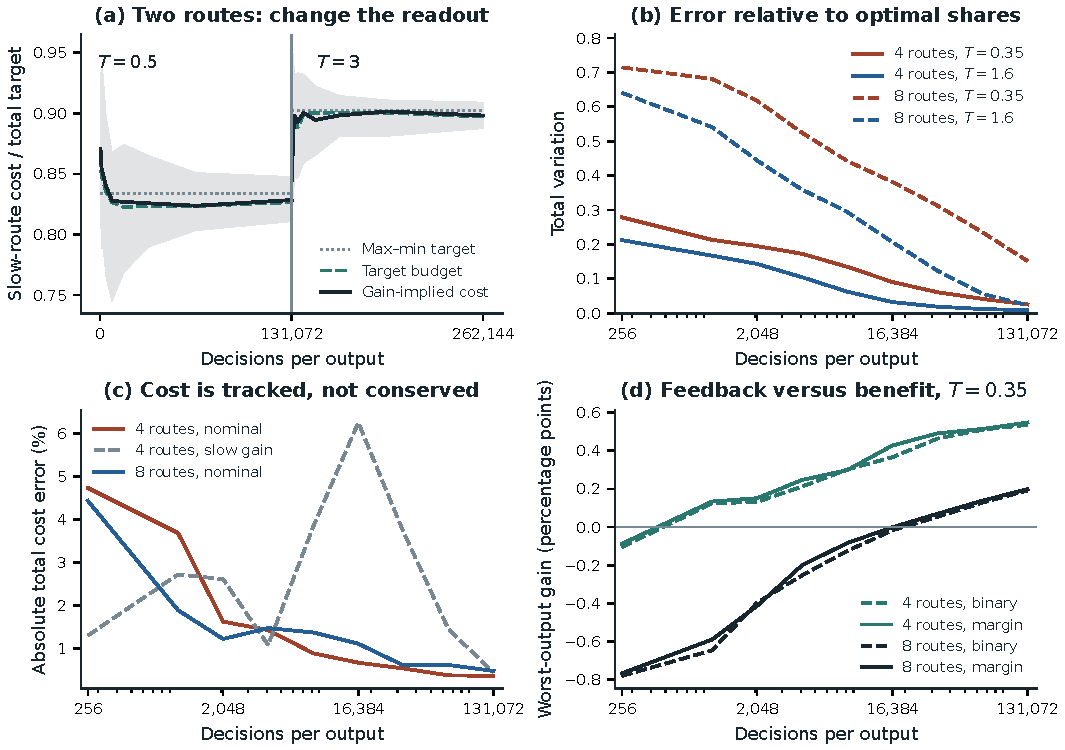
\includegraphics[width=\textwidth]{figures/fig_prrS_local_gain_loop.pdf}
\caption{\textbf{Activity-based gain regulation can follow a changing
readout, with finite-time allocation and cost errors.}
(a) In the two-route model, margin feedback redistributes the budget
after the window switch. Dotted gray shows the analytic optimum;
dashed teal shows target budget; solid dark shows frozen-gain cost.
The band is the 10th--90th percentile range across 48 realizations.
(b) Total variation from the optimal shares after normalizing the
gain-implied costs to sum to one. Solid: four routes; dashed: eight;
rust: short window; blue: long window. (c) Absolute error of the
gain-implied total cost relative to \(B\) at the short window. The
dashed gray curve uses a 64-fold slower actuator. (d) Change in
worst-output correctness evaluated at frozen gains, relative to the
unit-gain start. Dashed curves use binary feedback, solid curves
use cue-aligned margins. All curves are medians; each checkpoint
evaluates the second-half average of its run prefix.}
\label{fig:localgainloop}
\end{figure}

The model assigns functions to possible regulatory components:
neighbor comparisons transfer a conserved target resource and the
local filter tracks how strongly input fluctuations drive an output.
It assumes access to cue-free or separated source-driven activity,
evaluable task feedback, and a forward gain actuator that does not
modify the recurrent dynamics. It does not identify a biological
circuit that computes these quantities or maintains this resource.
